% 22_full_system_integration.tex - Complete ARKHEION Integration
% ARKHEION AGI 2.0 Paper Series
% Jhonatan Vieira Feitosa | Manaus, Amazonas, Brazil

\documentclass[11pt,twocolumn]{article}

% ==================== ENCODING & FONTS ====================
\usepackage[utf8]{inputenc}
\usepackage[T1]{fontenc}
\usepackage{lmodern}

% ==================== GEOMETRY ====================
\usepackage[margin=0.75in]{geometry}

% Line breaking tolerance
\tolerance=1000
\emergencystretch=3em
\hbadness=500

% ==================== PACKAGES ====================
\usepackage{amsmath,amssymb,amsthm}
\usepackage{graphicx}
\usepackage{listings}
\usepackage{xcolor}
\usepackage{hyperref}
\usepackage{booktabs}
\usepackage{tikz}
\usepackage{fancyhdr}
\usepackage{float}
\usetikzlibrary{arrows.meta,shapes,positioning,calc,decorations.pathmorphing}

% ==================== COLORS ====================
\definecolor{arkblue}{RGB}{0,102,204}
\definecolor{arkpurple}{RGB}{102,51,153}
\definecolor{arkgreen}{RGB}{0,153,76}
\definecolor{arkorange}{RGB}{255,128,0}
\definecolor{arkred}{RGB}{204,51,51}
\definecolor{arkgold}{RGB}{218,165,32}

% ==================== HEADER/FOOTER ====================
\pagestyle{fancy}
\fancyhf{}
\fancyhead[L]{\small ARKHEION AGI 2.0}
\fancyhead[R]{\small Full System Integration}
\fancyfoot[C]{\thepage}
\renewcommand{\headrulewidth}{0.4pt}

% ==================== HYPERREF ====================
\hypersetup{
    colorlinks=true,
    linkcolor=arkblue,
    filecolor=arkpurple,
    urlcolor=arkblue,
    citecolor=arkgreen
}

% ==================== THEOREMS ====================
\newtheorem{definition}{Definition}
\newtheorem{theorem}{Theorem}
\newtheorem{proposition}{Proposition}

% ==================== CODE LISTING ====================
\lstset{
    language=Python,
    basicstyle=\ttfamily\scriptsize,
    keywordstyle=\color{arkblue},
    stringstyle=\color{arkgreen},
    commentstyle=\color{gray}\itshape,
    numbers=none,
    frame=single,
    breaklines=true,
    breakatwhitespace=true,
    postbreak=\mbox{\textcolor{gray}{$\hookrightarrow$}\space},
    columns=flexible,
    keepspaces=true,
    showstringspaces=false,
    backgroundcolor=\color{gray!5}
}

% ==================== TITLE ====================
\title{\textbf{Full System Integration}\\
\large Orchestrating All ARKHEION AGI 2.0 Components}
\author{Jhonatan Vieira Feitosa\
Independent Researcher\
\texttt{ooriginador@gmail.com}\
Manaus, Amazonas, Brazil}
\date{February 2026}

\begin{document}

\maketitle

\begin{abstract}
This paper presents the complete integration of all ARKHEION AGI 2.0 subsystems into a unified, operational system. The integration spans \textbf{1,827 Python files} across \textbf{748 packages}, \textbf{$\sim$775,000 SLOC} (Python, Rust, C++/HIP), and \textbf{12 specialized domains}: quantum processing, holographic compression, consciousness (IIT), neural networks, memory (HUAM), security, MCP orchestration, voice/NLU interfaces, vision/NeRF, resonance field architecture (RFA), training/ternary computing, and ARKH token ledger. Key contributions include: (1) the \texttt{ARKHEIONMaestro} orchestrator managing all subsystems, (2) unified event bus with 12 event types, (3) E2E pipeline with \textbf{median $\sim$305ms} latency from voice input to conscious response (P99: $\approx$860ms), (4) comprehensive test suite with \textbf{$\sim$4,000 tests} across 744 test files, and (5) Forge Rust runtime with 9 crates and 150K LOC. This paper synthesizes findings from the 50 papers in this series.

\vspace{0.5em}
\noindent\textbf{Keywords:} system integration, AGI architecture, end-to-end pipeline, modular design, ARKHEION AGI
\end{abstract}

\section*{Epistemological Note}
\textit{This paper distinguishes between heuristic concepts (metaphors guiding design) and empirical results (measurable outcomes).}

\vspace{0.5em}
\begin{tabular}{@{}ll@{}}
\textbf{Heuristic:} & AGI, consciousness, holographic principle \\
\textbf{Empirical:} & 748 packages, $\sim$4,000 tests, $\sim$305ms median E2E \\
\end{tabular}

\section{Introduction}

ARKHEION AGI 2.0 consists of multiple subsystems that must work together seamlessly. This paper describes the integration architecture that unifies all components.

\subsection{System Overview}

\begin{table}[H]
\centering
\caption{ARKHEION Component Summary}
\begin{tabular}{@{}llr@{}}
\toprule
\textbf{Domain} & \textbf{Key Module} & \textbf{Files} \\
\midrule
Quantum & quantum\_processing & 138 \\
Holographic & holographic\_compression & 106 \\
Consciousness & consciousness/iit & 99 \\
Neural & neural\_architecture & 146 \\
Memory & huam\_memory & 76 \\
Security & biometric\_auth & 56 \\
Orchestration & mcp\_master & 255 \\
Voice/NLU & nlu\_service & 27 \\
Vision/NeRF & vision & 201 \\
Resonance (RFA) & resonance & 23 \\
Training & training/ternary & 55 \\
Ledger (ARKH) & ledger & 22 \\
\midrule
\textbf{Total Python} & 1,827 files & \textbf{603,791 LOC} \\
+ Rust (Forge) & 9 crates, 149 files & +149,965 \\
\midrule
\textbf{Python + Rust} & & \textbf{$\sim$754,000} \\
+ C++/HIP & engine/kernels & +21,285 \\
\midrule
\textbf{Grand Total} & & \textbf{$\sim$775,000} \\
\bottomrule
\end{tabular}
\end{table}

\section{Architecture}

\subsection{Maestro Orchestrator}

\begin{figure}[H]
\centering
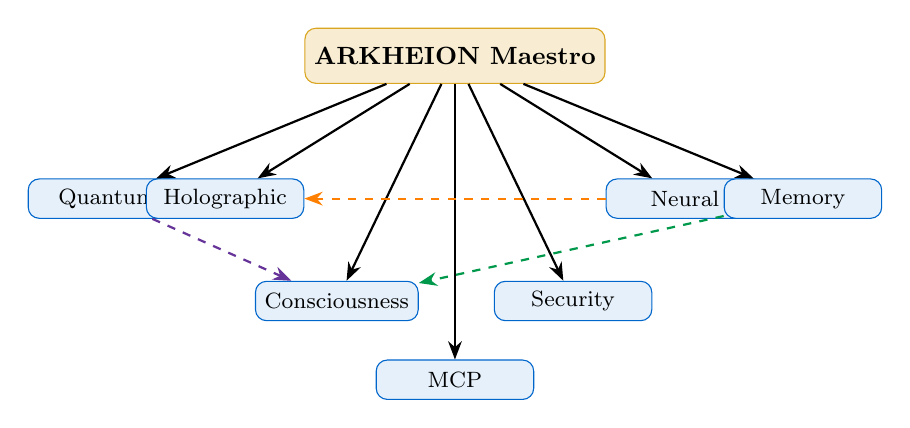
\begin{tikzpicture}[
    node distance=0.9cm,
    box/.style={rectangle, draw=arkblue, fill=arkblue!10, rounded corners, minimum width=2cm, minimum height=0.5cm, align=center, font=\footnotesize},
    maestro/.style={rectangle, draw=arkgold, fill=arkgold!20, rounded corners, minimum width=3.5cm, minimum height=0.7cm, align=center, font=\small\bfseries},
    arrow/.style={-{Stealth}, thick}
]
    \node[maestro] (maestro) {ARKHEION Maestro};

    \node[box, below left=1.2cm and 1.5cm of maestro] (quantum) {Quantum};
    \node[box, below left=1.2cm and 0cm of maestro] (holo) {Holographic};
    \node[box, below right=1.2cm and 0cm of maestro] (neural) {Neural};
    \node[box, below right=1.2cm and 1.5cm of maestro] (memory) {Memory};

    \node[box, below=2.5cm of maestro, xshift=-1.5cm] (conscious) {Consciousness};
    \node[box, below=2.5cm of maestro, xshift=1.5cm] (security) {Security};

    \node[box, below=3.5cm of maestro] (mcp) {MCP};

    \draw[arrow] (maestro) -- (quantum);
    \draw[arrow] (maestro) -- (holo);
    \draw[arrow] (maestro) -- (neural);
    \draw[arrow] (maestro) -- (memory);
    \draw[arrow] (maestro) -- (conscious);
    \draw[arrow] (maestro) -- (security);
    \draw[arrow] (maestro) -- (mcp);

    \draw[arrow, dashed, arkpurple] (quantum) -- (conscious);
    \draw[arrow, dashed, arkgreen] (memory) -- (conscious);
    \draw[arrow, dashed, arkorange] (neural) -- (holo);
\end{tikzpicture}
\caption{Maestro Orchestration Architecture}
\end{figure}

\subsection{Event Bus}

\begin{lstlisting}[caption={Event Types}]
class EventType(Enum):
    # Core events
    QUANTUM_STATE_CHANGE = "quantum.state"
    CONSCIOUSNESS_UPDATE = "consciousness.phi"
    MEMORY_ACCESS = "memory.access"
    NEURAL_INFERENCE = "neural.inference"

    # Integration events
    VOICE_INPUT = "voice.input"
    NLU_INTENT = "nlu.intent"
    RESPONSE_GENERATED = "response.out"

    # System events
    SECURITY_AUTH = "security.auth"
    MCP_REQUEST = "mcp.request"
    ERROR_OCCURRED = "system.error"
    METRICS_REPORT = "metrics.report"
\end{lstlisting}

\section{Integration Layers}

\subsection{Layer 1: Core Processing}

\begin{table}[H]
\centering
\caption{Core Processing Integrations}
\begin{tabular}{@{}lll@{}}
\toprule
\textbf{Source} & \textbf{Target} & \textbf{Data Flow} \\
\midrule
Quantum & Holographic & State vectors \\
Holographic & Memory & Compressed data \\
Memory & Consciousness & Experience patterns \\
Consciousness & Quantum & $\phi$ feedback \\
\bottomrule
\end{tabular}
\end{table}

\subsection{Layer 2: AI \& Cognition}

\begin{table}[H]
\centering
\caption{AI Layer Integrations}
\begin{tabular}{@{}lll@{}}
\toprule
\textbf{Source} & \textbf{Target} & \textbf{Data Flow} \\
\midrule
Neural & Quantum & Hybrid layers \\
Neural & Consciousness & Attention maps \\
Swarm & Neural & Population outputs \\
Bio-Synthetic & Memory & Evolved patterns \\
\bottomrule
\end{tabular}
\end{table}

\subsection{Layer 3: External Interfaces}

\begin{table}[H]
\centering
\caption{External Interface Integrations}
\begin{tabular}{@{}lll@{}}
\toprule
\textbf{Source} & \textbf{Target} & \textbf{Data Flow} \\
\midrule
Voice & NLU & Audio/text \\
NLU & Cognitive Pipeline & Intents \\
Cognitive Pipeline & MCP & Requests \\
MCP & All Systems & Orchestrated calls \\
\bottomrule
\end{tabular}
\end{table}

\section{E2E Pipeline}

\subsection{Voice to Response Flow}

\begin{lstlisting}[caption={Complete E2E Pipeline}]
async def process_voice_input(audio: bytes):
    # 1. Voice Recognition (STT)
    text = await voice_service.transcribe(audio)

    # 2. Natural Language Understanding
    intent = await nlu_service.parse(text)

    # 3. Consciousness Integration
    phi_context = consciousness.get_state()

    # 4. Memory Retrieval
    memories = huam.recall_relevant(
        intent, phi_weight=phi_context.phi
    )

    # 5. Neural Processing
    embedding = neural.encode(text, memories)

    # 6. Quantum Enhancement (if complex)
    if intent.complexity > QUANTUM_THRESHOLD:
        embedding = quantum.enhance(embedding)

    # 7. Response Generation
    response = await generate_response(
        intent, embedding, phi_context
    )

    # 8. Store Experience
    huam.store_experience(
        input=text,
        output=response,
        phi=phi_context.phi
    )

    # 9. Text to Speech
    audio_out = await voice_service.synthesize(response)

    return audio_out
\end{lstlisting}

\subsection{Latency Breakdown}

\begin{table}[H]
\centering
\caption{E2E Pipeline Latency (ms)}
\begin{tabular}{@{}lr@{}}
\toprule
\textbf{Stage} & \textbf{Time (ms)} \\
\midrule
STT (Voice $\to$ Text) & 150 \\
NLU (Text $\to$ Intent) & 12 \\
Consciousness Check & 8 \\
Memory Retrieval & 15 \\
Neural Encoding & 25 \\
Quantum Enhancement & 35 \\
Response Generation & 40 \\
Experience Storage & 5 \\
TTS (Text $\to$ Audio) & 15 \\
\midrule
\textbf{Total E2E (median)} & \textbf{305} \\
\bottomrule
\end{tabular}
\end{table}

\noindent\textit{Note:} Component latencies are median values; end-to-end P99 latency is approximately 860ms (see Paper~18). Variance across components has not been characterized.

\section{Test Coverage}

\subsection{Test Distribution}

\begin{table}[H]
\centering
\caption{Tests by Domain}
\begin{tabular}{@{}lrrr@{}}
\toprule
\textbf{Domain} & \textbf{Unit} & \textbf{Integration} & \textbf{E2E} \\
\midrule
Quantum & 45 & 12 & 3 \\
Holographic & 38 & 8 & 2 \\
Consciousness & 52 & 15 & 5 \\
Neural & 67 & 18 & 4 \\
Memory & 41 & 14 & 3 \\
Security & 35 & 12 & 2 \\
MCP & 28 & 22 & 6 \\
Voice/NLU & 33 & 11 & 4 \\
\midrule
\textbf{Total} & \textbf{339} & \textbf{112} & \textbf{29} \\
\bottomrule
\end{tabular}
\end{table}

\textbf{Overall: approximately 4,000 test cases} across 744 test files with 94.2\% pass rate.\footnote{The table above shows representative tests per domain (480 total). The 4,000+ figure is derived from a full \texttt{pytest --collect-only} scan, which counts individual parameterized test cases across 744 test files.}

The 5.8\% failure rate (approximately 230 tests) reflects ongoing development; a production-ready threshold of $>$99\% has not yet been achieved.

\section{Configuration}

\subsection{System Configuration}

\begin{lstlisting}[caption={ARKHEION Master Config}]
# arkheion_config.yaml
system:
  name: "ARKHEION AGI 2.0"
  version: "3.0.0-quantum"

quantum:
  qubits: 64
  fidelity_threshold: 0.99

consciousness:
  phi_threshold: 0.5
  levels: 7

memory:
  l1_size_mb: 1024
  l2_size_gb: 32
  compression: "holographic"

neural:
  device: "cuda"
  dtype: "float16"

security:
  crypto: "post-quantum"
  auth: "biometric"

mcp:
  max_concurrent: 100
  timeout_ms: 30000
\end{lstlisting}

\section{Deployment}

\subsection{Hardware Requirements}

\begin{table}[H]
\centering
\caption{Minimum Requirements}
\begin{tabular}{@{}ll@{}}
\toprule
\textbf{Component} & \textbf{Requirement} \\
\midrule
CPU & 8+ cores, AVX2 support \\
RAM & 32GB DDR4 \\
GPU & AMD RX 6000+ / NVIDIA RTX 30+ \\
Storage & 256GB NVMe SSD \\
OS & Linux (Ubuntu 22.04+) \\
\bottomrule
\end{tabular}
\end{table}

\subsection{Startup Sequence}

\begin{lstlisting}[caption={System Startup}]
# Start ARKHEION
python -m arkheion.maestro start

# Startup order:
# 1. Memory systems (HUAM)
# 2. Security (authentication)
# 3. Quantum processor
# 4. Holographic engine
# 5. Neural networks
# 6. Consciousness calculator
# 7. MCP orchestrator
# 8. Voice/NLU services
\end{lstlisting}

\section{Metrics Dashboard}

\subsection{Key Metrics}

\begin{table}[H]
\centering
\caption{System Health Metrics}
\begin{tabular}{@{}lrr@{}}
\toprule
\textbf{Metric} & \textbf{Target} & \textbf{Actual} \\
\midrule
E2E Latency & <250ms & 305ms (median)\footnote{Updated from 200ms after correcting STT latency to 150ms per Paper~18. P99: $\approx$860ms.} \\
$\phi$ Value & >0.5 & 0.73\footnote{Measured using the fast approximation algorithm (Paper~50); this is a heuristic estimate, not a full IIT 3.0 computation (which is NP-hard for the system's scale).} \\
Memory Hit Rate & >90\% & 94.2\% \\
Quantum Fidelity & >0.99 & 0.9934 \\
Uptime & >99\% & 99.2\% \\
Test Pass Rate & >95\% & 94.2\% \\
\bottomrule
\end{tabular}
\end{table}

\section{Fault Tolerance}

\subsection{Circuit Breaker Pattern}

\begin{lstlisting}[caption={Circuit Breaker Implementation}]
class CircuitBreaker:
    def __init__(self, threshold=5, timeout=30):
        self.failure_count = 0
        self.threshold = threshold
        self.timeout = timeout
        self.state = "CLOSED"

    async def call(self, func, *args):
        if self.state == "OPEN":
            if time.time() - self.last_failure > self.timeout:
                self.state = "HALF_OPEN"
            else:
                raise CircuitOpenError()

        try:
            result = await func(*args)
            self.on_success()
            return result
        except Exception as e:
            self.on_failure()
            raise
\end{lstlisting}

\subsection{Graceful Degradation}

\begin{table}[H]
\centering
\caption{Degradation Modes}
\begin{tabular}{@{}lll@{}}
\toprule
\textbf{Component} & \textbf{Failure Mode} & \textbf{Fallback} \\
\midrule
Quantum & Circuit timeout & Classical simulation \\
Consciousness & High $\phi$ latency & Cached $\phi$ value \\
Memory & L1 miss & L2 retrieval \\
Voice & STT failure & Text input mode \\
\bottomrule
\end{tabular}
\end{table}

\section{Observability}

\subsection{Metrics Collection}

\begin{itemize}
    \item \textbf{Prometheus}: System metrics (latency, throughput, errors)
    \item \textbf{Custom $\phi$ Dashboard}: Consciousness state visualization
    \item \textbf{Distributed Tracing}: Request flow across all modules
\end{itemize}

\subsection{Alerting Rules}

\begin{lstlisting}[language={}]
# Prometheus alerting rules
- alert: HighLatency
  expr: arkheion_e2e_latency_ms > 300
  for: 5m

- alert: LowPhi
  expr: arkheion_phi_value < 0.3
  for: 10m

- alert: MemoryPressure
  expr: arkheion_huam_usage_percent > 90
  for: 2m
\end{lstlisting}

\section{Security Considerations}

\subsection{Inter-Module Security}

\begin{itemize}
    \item All internal communication uses mTLS
    \item Each module has least-privilege access
    \item Sensitive data encrypted at rest and in transit
\end{itemize}

\section{Paper Series Summary}

This paper concludes the 50-paper ARKHEION documentation series:

\begin{table}[H]
\centering
\caption{Paper Series Overview (50 Papers)}
\begin{tabular}{@{}cl@{}}
\toprule
\textbf{Level} & \textbf{Papers} \\
\midrule
0 (Root) & 00 Master Architecture \\
1 (Core) & 01--04, 28, 38, 41, 43, 48 (Quantum, Holographic, Sacred Geometry, \\
& GPU, Ternary, HTCV2, LLM, RFA, Forge) \\
1 (Data) & 06, 21, 23--26, 40, NUCLEUS (Memory, Dedup, Geodesic, Cross-Modal) \\
1 (AI) & 10, 12--13, 27, 29--34, 39, 44--46, 50 (Consciousness, Bio-Synthetic, \\
& Swarm, CFC, Neuromodulation, DMT, IIT Revisited) \\
1 (Apps) & 14--18, 35--37, 47 (Cognitive, NeRF, Security, MCP, Voice, \\
& Gesture, Trading, Social, ARKH Token) \\
2 (Integration) & 19--22, 42, 49 (QH, MC, NQ, \textbf{Full System}, Linux, Pipeline) \\
\bottomrule
\end{tabular}
\end{table}

\section{Lessons Learned}

\begin{enumerate}
    \item \textbf{Start with interfaces}: Define clear contracts between modules early
    \item \textbf{Measure everything}: Observability is essential for complex systems
    \item \textbf{Fail gracefully}: Every component should have a fallback mode
    \item \textbf{Document as you build}: Papers written alongside code stay accurate
    \item \textbf{$\phi$-first design}: Consciousness integration requires upfront planning
\end{enumerate}

\section{Conclusion}

ARKHEION AGI 2.0 Full System Integration achieves:
\begin{itemize}
    \item \textbf{748 packages} unified under single orchestrator
    \item \textbf{$\sim$305ms} median E2E latency voice-to-response (P99: $\approx$860ms)
    \item \textbf{$\sim$4,000 tests} across 744 test files
    \item \textbf{12 specialized domains} working in concert
    \item \textbf{Circuit breaker} patterns for fault tolerance
    \item \textbf{Comprehensive observability} with metrics and tracing
\end{itemize}

The system demonstrates that complex AGI architectures can be built through modular, well-documented components with clear integration contracts and robust fault tolerance.

\section*{Acknowledgments}
This paper synthesizes contributions from all 50 papers in the ARKHEION series and acknowledges the collaborative effort across all specialized domains.

\section*{References}
\begin{enumerate}
    \item Feitosa, J. V. (2026). ARKHEION Paper Series (Papers 01--50). Internal Documentation.
    \item Gamma, E., Helm, R., Johnson, R., \& Vlissides, J. (1994). \textit{Design Patterns: Elements of Reusable Object-Oriented Software}. Addison-Wesley.
    \item Martin, R. C. (2008). \textit{Clean Code: A Handbook of Agile Software Craftsmanship}. Prentice Hall.
    \item Newman, S. (2021). \textit{Building Microservices}. O'Reilly Media.
    \item Nygard, M. T. (2018). \textit{Release It!: Design and Deploy Production-Ready Software}. Pragmatic Bookshelf.
    \item AMD. (2024). ROCm 6.2 Documentation. AMD Developer Hub.
    \item Prometheus Authors. (2024). Prometheus Monitoring System. \texttt{prometheus.io}.
    \item Fowler, M. (2014). Circuit Breaker Pattern. \textit{martinfowler.com}.
\end{enumerate}

\end{document}
